\chapter{Preliminaries and Introduction\label{sec:introduction}}

\section{Introduction}
The theme of our idea is to use most advance technology and the naïve and good people of our country together as a whistle-blower to save the country from crime.  The main focus of our system is to ensure the safety of the whistle-blowers. Because increase in crime day by day we don’t know who is corrupt or not in the system.\\
The focus on blockchain technology is to make people unknown to each other in this application of ours. Which will ensure the safety of the people real time. The cases can be of any region all around the country. People can view all the cases and if you have something regarding that case you can go and register as a Whistle-Blower and submit the evidence regarding that case which will be viewed by the Police and Jury. Once the assessment has been made, can perform execution.\\
The Police Officer and Whistle-Blower both are unknown to each other. And both will be rewarded.   The figure below (see \figref{tst}) shows an example of Whistle-Blower.\\
\begin{figure}[h]
	\centering
	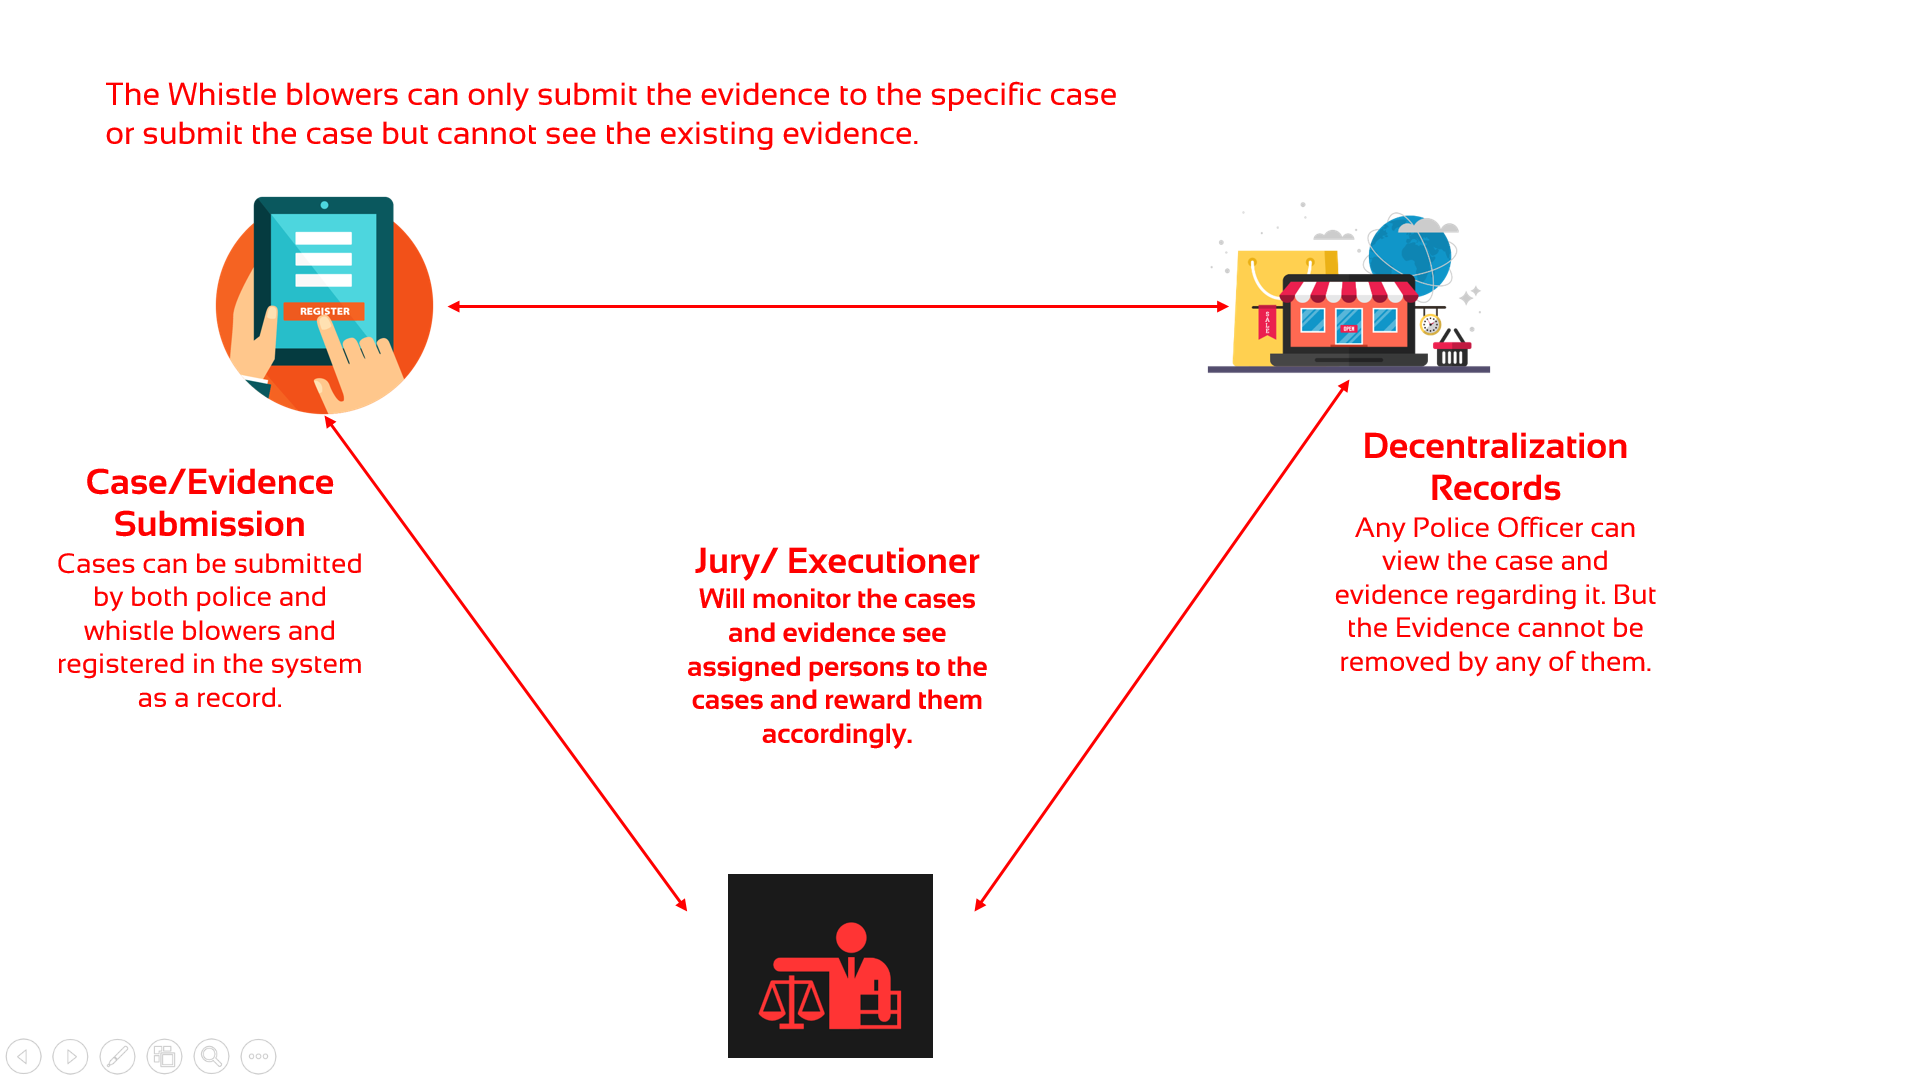
\includegraphics[scale=0.40]{figures/01.png}
	\caption{Whistle-Blower}
	\label{fig:ist}
\end{figure}
 The working or idea of this project \figref{ist} is that a whistle-Blower go to the website and submit those cases that are not been already upload that shown in figure.
\begin{figure}[h]
	\centering
	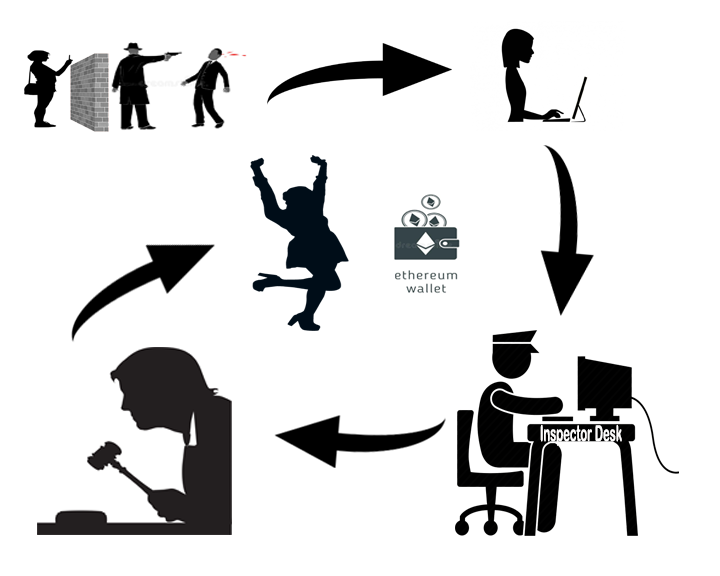
\includegraphics[width=0.50\textheight]{figures/02.png}
	\caption{Overview of Whistle-Blower}
	\label{fig:tst}
\end{figure}
In the \figref{tst}, we have Whole \textbf{ Overview } of the Whistle-Blower project that insure the security of the Person who become part of our project.\\

\subsection{Cases}
Currently we are only dealing with CORRUPTION cases only, but the system should be robust enough to accommodate other crimes in the future. The biggest challenge with the system in place is lack of rewarding mechanism and that cases are mostly mishandled and investigators are easily compromised by the perpetrators, once investigators are compromised they end up tampering with evidence and later on claiming that there wasn’t sufficient evidence. They also use delay tactics to buy time till the members of the media and members of the public has forgotten about the cases (with a work-flow based blockchain system, every step of the case will be in the public Domain and the system can even generate automated reports to show the duration each case has been at a certain stage). The investigators also start blaming the judiciary for poor verdict after cases have dragged for years and years yet mostly it’s them who door a poor job in collecting evidence. That’s why it’s important to have a system that keeps checking what’s happening at every stage of the case and who has failed the country in the fight against corruption. Rewarding mechanism is also key to make sure that there’s incentive to investigators and whistle blowers.\\
Sub categories within corruption related crimes include the following:
\begin{itemize}
	\item Conflict of interest Info / Explanation Conflict of interest
	\item  Bribery Info / Explanation Bribery
	\item  Fraud Info / Explanation Fraud
	\item  Land grabbing Info / Explanation Land grabbing
	\item  Breach of trust Info / Explanation Breach of trust
	\item  Tax evasion
		
\end{itemize}
The system should be able to assign cases to specific investigators/police based on certain rules set in the system. Investigators/police should only see cases they are dealing with or cases assigned to them. This will ensure that investigators can be held responsible for every aspect of the case without blaming their colleagues if investigation is compromised at some point.
\subsection{Corruption Sub Categories Include}
\subsubsection{Conflict Of Interest}

A conflict of interest is a situation in which a public officer has a private interest in a matter that concerns his office and he fails to disclose the private interest to his employer.
It is not an offense if the public officer has disclosed his interest and has been allowed to participate in the decision making process.\\
Some examples:\\
Self-dealing: A public officer doing a business with an organization which he works for without disclosing
Outside employment: Somebody holding two jobs in which the interest of one job conflicts with the other without disclosing

A public officer employing or giving services to a family member, relative or friends without disclosing
Gifts: Gifts from friends who also do business with the person receiving the gifts without disclosing (Such gifts may include things of value such as transportation and lodging).


\subsubsection{Bribery}
Giver: To promise, offer, or give something of value to a person in order to obtain services or gain influence; or\\
Recipient: To receive or demand, or agree to acquire or ask a private benefit so as to provide public services/goods.\\
Private benefit: gift, loan, fee, reward, appointment, service, favor, failure to take action, promise or other consideration or advantage.\\
Some examples:\\
Offering / Giving something of value
Agreeing to offer / give something of value
Demanding for / receiving a private benefit
\subsubsection{Fraud}
The action or instance of deception for financial or personal gain or so as to obtain goods or services illegally.\\
Some examples:\\

\begin{itemize}
	\item Conversion of organization’s property for personal use
	\item Falsification of documents
	\item Over valuing or under valuing of goods
	\item Conversion of organization’s property for personal use
\end{itemize}

\subsubsection{Abuse of Office}
A person who uses his office to improperly benefit oneself or another person.\\
Some examples:\\
\begin{itemize}
	\item breach of procurement rules to favour somebody
	\item Nepotism
	\item favouritism
	\item abuse of discretion / power
	
\end{itemize}

\subsubsection{Land Grabbing}
Fraudulent acquisition and disposal of public land. This includes to illegally acquire, sell, transfer, lease, charge or mortgage OR in any way dispose of public land.\\
Some examples:\\
Land set aside for public utilities such as\\


\begin{itemize}
	\item schools
	\item dispensary/hospitals
	\item road reserves and parking bays
	\item public toilets
\end{itemize}



\subsubsection{Breach of Trust}
Failure to honour a responsibility of trust and confidence bestowed upon a person by virtue of his office.\\
Some examples:\\
\begin{itemize}
	\item Where managers of pension funds have irregularly invested member funds in breach of laid down regulations
	\item Irregular investment of public funds in breach of regulations
	\item Mismanagement by appointed administrators and executors of property entrusted under their care
	\item Mismanagement of property by receiver managers / liquidators etc.

\end{itemize}



\subsection{Selected Use Cases of Application}
The main feature of our application is:
\subsubsection{Registration of Whistle-Blower}

The whistle-blowers are going to register to our system using a wallet number. If you don’t have a wallet number you can go to any crypto currency site and get one. If you want to use fiat currency, scatter wallet is also a good option. Using online wallets is because they does not trace back to you easily. Once the whistle blower is registered its wallet number will be shown only to the Jury. He/she will submit the evidence and that’s it. They also cannot see the evidence that’s already been there uploaded by the other people.
   
\subsubsection{Registration of Police Officer}

The registration of Police Officer will also be done by the same process. A wallet number and the police ID number original given by the Police Department will be used to register. If the case is uploaded by the police officer and also in his jurisdiction, he is the in charge of that case else we have to look for the regional officer where the incident happen.  

\subsubsection{Submission of Evidence/Case by Whistle-Blower/ Police Officer}
There is a general interface view of all the running cases. A criminal can also see that. But he can also be a whistle blower and see the evidence against that case. That’s why we have removed jurisdiction of anyone except police and jury to see the evidence. You can only submit the evidence and case. Cases and evidence both can be uploaded by anyone in the country. 

\subsubsection{Agency/Judge monitoring them both}
To avoid corruption and crime completely, we are introducing the jury system which will monitor the both the cases and the evidence and ask questions that what is the progress on that case. The jury will be selected very carefully and there will be more than one person so they cannot be bought. 
\subsubsection{Pending Cases}
The duration will be assigned to every single case. If the cases are older than three month, they will be shown on a separated case. 
\subsubsection{A Reward System}
If the evidence or case submitted by the police or whistle blower and finished successfully, both the police officer and the whistle blower will be awarded. These is a kind of small amount in the form of a currency. 


\subsection{How This will solve the problem through use of the blockchain}
The solution applies blockchain technology to overcome many problems around the cost, flexibility, and scalability of business support systems faced by old crime reporting systems, and to provide extensive opportunities to enhance product offerings and whistle blower experience. \\
A shared view – The Police and Judge both parties can inspect the cases fully and perform queries. People can search on the basis of region, categories, age of the case. \\
New cases and evidence – It has the ability to handle large amount of data. Its blockchain back end so if memory runs out we can simply use external cloud storage like IPFS. \\ 
Easy Reward – The Police Officer and whistle blower will be rewarded through a wallet ID by the jury.  \\
Easy and instant secure payments – The payments done will be 100 perent secure no traces back to its original owner, ensuring the safety of all the whistle blowers.   \\
A scalable solution – freeing the billing and contracting processing from physical hardware and constraints significantly improves the Operators ability to scale to explore new expansion opportunities. \\
The flexibility to respond to changing conditions – the contract mechanism give the administrator and jury the ability to change the contract to meet new upcoming challenges. \\ 
Confidential and secure client contracts – Using consortium blockchain technology i.e. per-missioned and private decentralized ledgers, the data submitted will be 100 confidential.\\ 
Secure communications – The DApp shall be securely connecting the Smart contract with the Police and whistle blower interface.  

